\documentclass[11pt,a4paper]{article}
\usepackage[margin=1.8cm]{geometry}
\usepackage{tikz}
\usetikzlibrary{calc,intersections,angles,quotes}
\usepackage{multicol}
\usepackage{enumitem}
\usepackage{amsmath,amssymb}
\setlength{\parskip}{0.6em}
\setlength{\parindent}{0pt}

\newcommand{\Title}{Angles in the Same Segment — Worksheet}

% --- TikZ styles & colors ---
\definecolor{segmentblue}{RGB}{200,220,255}
\definecolor{sectororange}{RGB}{255,220,180}
\definecolor{lightgray}{RGB}{230,230,230}
\definecolor{segmentgreen}{RGB}{210,250,210}
\definecolor{segmentpurple}{RGB}{235,210,255}
\definecolor{sectoryellow}{RGB}{255,245,180}

\tikzset{
  chord/.style={thick},
  circleline/.style={thick},
  point/.style={fill=black, circle, inner sep=1.2pt},
  anglemark/.style={draw, thick},
  labelAB/.style={font=\small}
}

% --- Adjustable radii ---
\def\Rmini{1.6}
\def\Rwork{2.2}
\def\Rlarge{3.0}

% --- Utilities: coordinates on a circle ---
% Usage: \coordOnCircle{<name>}{<R>}{<deg>}
\newcommand{\coordOnCircle}[3]{%
  \coordinate (#1) at ({#2*cos(#3)},{#2*sin(#3)});
}

% --- Draw a shaded SEGMENT between A(angle a) and B(angle b) on a circle of radius R, centered at origin in a shifted scope ---
% Assumes a<b and minor segment desired.
% Options: label=1 to label A,B; chord=1 to draw chord; arc=1 to draw circle outline
\newcommand{\SegmentShaded}[9]{%
  % #1 x-shift, #2 y-shift, #3 R, #4 angA, #5 angB, #6 drawChord(0/1), #7 drawCircle(0/1), #8 labelAB(0/1), #9 fill color
  \begin{scope}[shift={(#1,#2)}]
    % Circle and points
    \draw[circleline, opacity=0.7] (0,0) circle (#3);
    \coordOnCircle{A}{#3}{#4}
    \coordOnCircle{B}{#3}{#5}
    % Segment fill
    \fill[#9] (A) arc[start angle=#4, end angle=#5, radius=#3] -- (B) -- cycle;
    % Optional circle outline stronger
    \ifnum#7>0
      \draw[circleline] (0,0) circle (#3);
    \fi
    % Optional chord
    \ifnum#6>0
      \draw[chord] (A)--(B);
    \fi
    % Optional labels
    \ifnum#8>0
      \node[labelAB, below right=1pt of A] {\(A\)};
      \node[labelAB, below left=1pt of B] {\(B\)};
      \fill (A) circle (1pt);
      \fill (B) circle (1pt);
    \fi
  \end{scope}
}

% --- Draw a shaded SECTOR (center-to-arc wedge) between A and B ---
\newcommand{\SectorShaded}[9]{%
  % #1 x-shift, #2 y-shift, #3 R, #4 angA, #5 angB, #6 drawRadii(0/1), #7 drawCircle(0/1), #8 labelAB(0/1), #9 fill color
  \begin{scope}[shift={(#1,#2)}]
    \draw[circleline, opacity=0.7] (0,0) circle (#3);
    \coordOnCircle{A}{#3}{#4}
    \coordOnCircle{B}{#3}{#5}
    \fill[#9] (0,0) -- (A) arc[start angle=#4, end angle=#5, radius=#3] -- cycle;
    \ifnum#7>0
      \draw[circleline] (0,0) circle (#3);
    \fi
    \ifnum#6>0
      \draw[chord] (0,0)--(A);
      \draw[chord] (0,0)--(B);
    \fi
    \ifnum#8>0
      \node[labelAB, below right=1pt of A] {\(A\)};
      \node[labelAB, below left=1pt of B] {\(B\)};
      \fill (A) circle (1pt);
      \fill (B) circle (1pt);
    \fi
  \end{scope}
}

% --- Draw a CHORD-ONLY picture (no shading) ---
\newcommand{\ChordOnly}[6]{%
  % #1 x-shift, #2 y-shift, #3 R, #4 angA, #5 angB, #6 labelAB(0/1)
  \begin{scope}[shift={(#1,#2)}]
    \draw[circleline] (0,0) circle (#3);
    \coordOnCircle{A}{#3}{#4}
    \coordOnCircle{B}{#3}{#5}
    \draw[chord] (A)--(B);
    \ifnum#6>0
      \node[labelAB, below right=1pt of A] {\(A\)};
      \node[labelAB, below left=1pt of B] {\(B\)};
      \fill (A) circle (1pt);
      \fill (B) circle (1pt);
    \fi
  \end{scope}
}

% --- Theorem picture: equal angles in same segment (left) and blank circle to shade (right) ---
\newcommand{\TheoremPair}[9]{%
  % Left diagram (angles shown)
  % #1 x-left, #2 y, #3 R, #4 angA, #5 angB, #6 angC, #7 angD, #8 x-right offset, #9 title label (e.g., (a))
  \begin{scope}[shift={(#1,#2)}]
    \node[anchor=west, font=\bfseries] at (-0.2-#3, #3+0.7) {#9};
    \draw[circleline] (0,0) circle (#3);
    \coordOnCircle{A}{#3}{#4}
    \coordOnCircle{B}{#3}{#5}
    \coordOnCircle{C}{#3}{#6}
    \coordOnCircle{D}{#3}{#7}
    \draw[chord] (A)--(B);
    % Angles ACB and ADB
    \draw (A)--(C)--(B);
    \draw (A)--(D)--(B);
    % Mark equal angles
    \pic[draw, angle eccentricity=1.2, angle radius=0.5cm] {angle = A--C--B};
    \pic[draw, angle eccentricity=1.2, angle radius=0.5cm] {angle = A--D--B};
    % Optional labels
    \fill (A) circle (1pt);
    \fill (B) circle (1pt);
    \fill (C) circle (1pt);
    \fill (D) circle (1pt);
  \end{scope}
  % Right companion (blank circle with same chord for shading task)
  \begin{scope}[shift={({#1 + #8},#2)}]
    \draw[circleline] (0,0) circle (#3);
    \coordOnCircle{A2}{#3}{#4}
    \coordOnCircle{B2}{#3}{#5}
    \draw[chord] (A2)--(B2);
    \fill (A2) circle (1pt);
    \fill (B2) circle (1pt);
  \end{scope}
}

\begin{document}
\begin{center}
  {\LARGE \bfseries \Title}\\[0.25em]
  \small Angles subtended by the same chord at the circumference, in the same segment, are equal.
\end{center}

\hrule
\vspace{2em}

\textbf{1) Identify the segments.}  
In each diagram below, decide whether the \emph{shaded} region is a \textbf{segment}, a \textbf{sector}, or neither (e.g.\ just a chord).  
Tick the ones that are \textbf{segments}. 

\vspace{0.6em}
\begin{center}
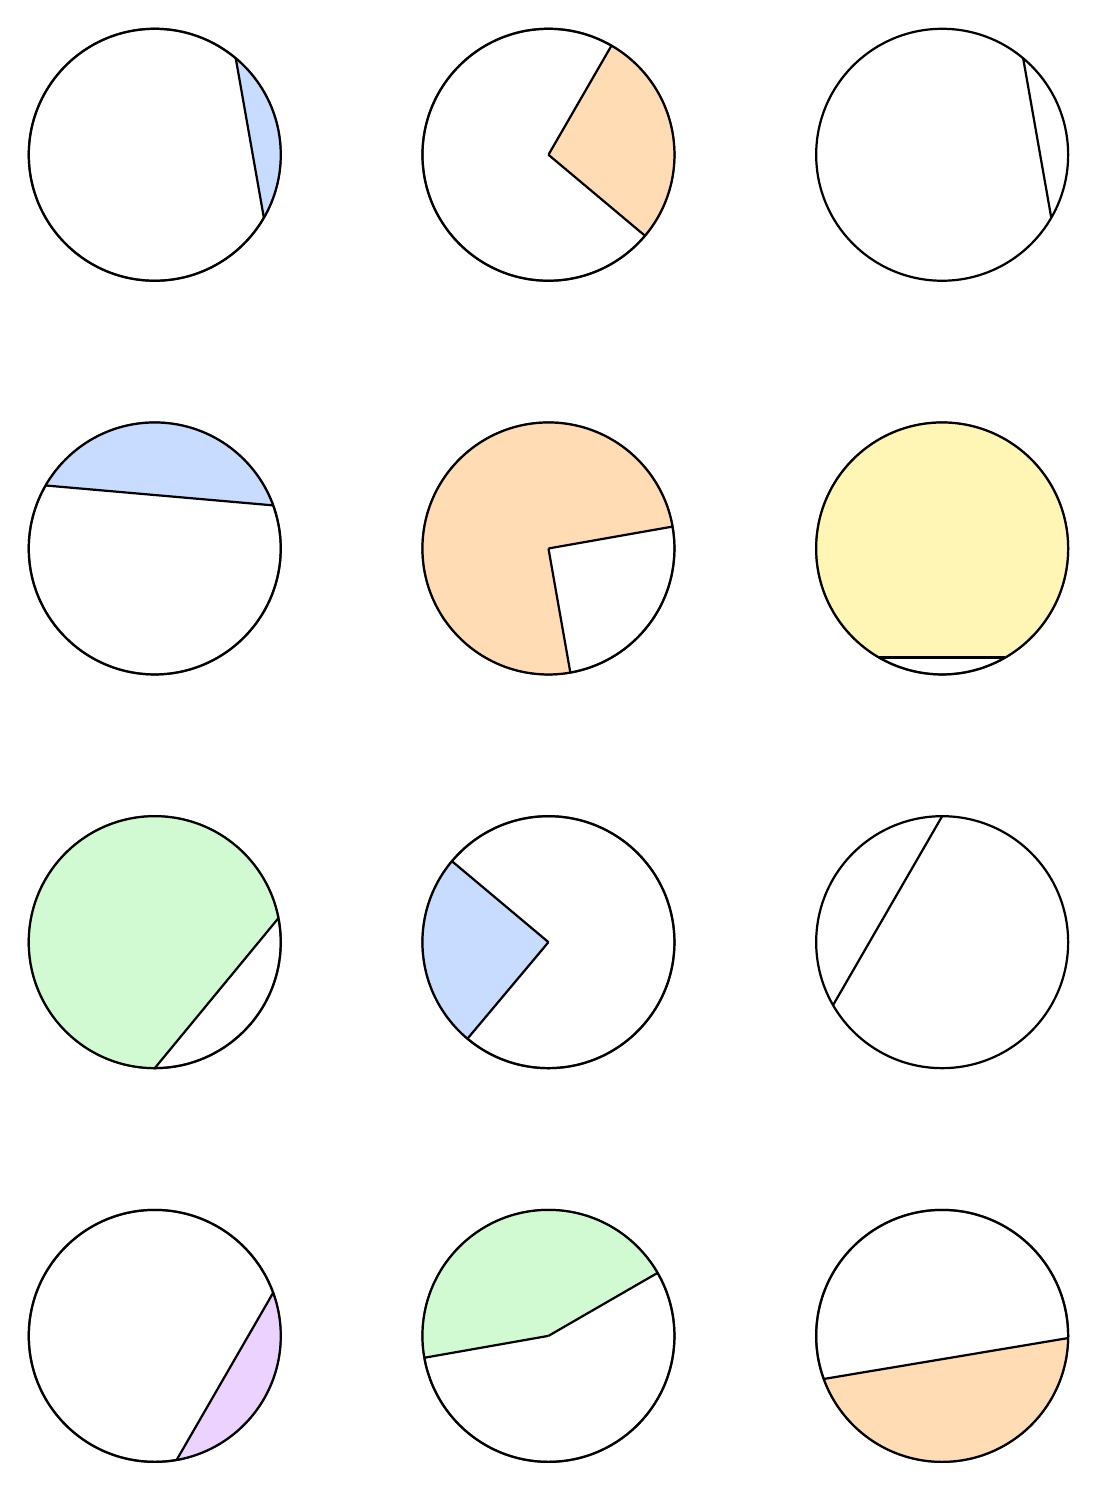
\begin{tikzpicture}[scale=1]

  % =======================
  % Row 1 (original)
  % =======================
  \SegmentShaded{-6.8}{0}{\Rmini}{-30}{50}{1}{1}{0}{segmentblue}
  \SectorShaded{-1.8}{0}{\Rmini}{-40}{60}{1}{1}{0}{sectororange}
  \ChordOnly{3.2}{0}{\Rmini}{-30}{50}{0}

  % =======================
  % Row 2 (original, one angle corrected)
  % =======================
  \SegmentShaded{-6.8}{-5}{\Rmini}{20}{150}{1}{1}{0}{segmentblue}
  \SectorShaded{-1.8}{-5}{\Rmini}{280}{10}{1}{1}{0}{sectororange}
  \SegmentShaded{3.2}{-5}{\Rmini}{-60}{240}{1}{1}{0}{sectoryellow}

  % =======================
  % Row 3 (new colours)
  % =======================
  \SegmentShaded{-6.8}{-10}{\Rmini}{270}{11}{1}{1}{0}{segmentgreen}
  \SectorShaded{-1.8}{-10}{\Rmini}{140}{230}{1}{1}{0}{segmentblue}
  \ChordOnly{3.2}{-10}{\Rmini}{90}{210}{0}

  % =======================
  % Row 4 (new colours)
  % =======================
  \SegmentShaded{-6.8}{-15}{\Rmini}{-80}{20}{1}{1}{0}{segmentpurple}
  \SectorShaded{-1.8}{-15}{\Rmini}{30}{190}{1}{1}{0}{segmentgreen}
  \SegmentShaded{3.2}{-15}{\Rmini}{200}{359}{1}{1}{0}{sectororange}

\end{tikzpicture}
\end{center}

\newpage{}

\textbf{2) Draw angles in a given segment.}  
In each circle, the \textbf{segment} has been shaded.  
\emph{Draw angles at the circumference} in the shaded segment.
\begin{enumerate}[label=(\alph*)]
  \item Draw \textbf{1} angle.
  \item Draw \textbf{2} different angles.
  \item Draw \textbf{3} different angles.
  \item Draw \textbf{10} different angles.
\end{enumerate}

\begin{center}
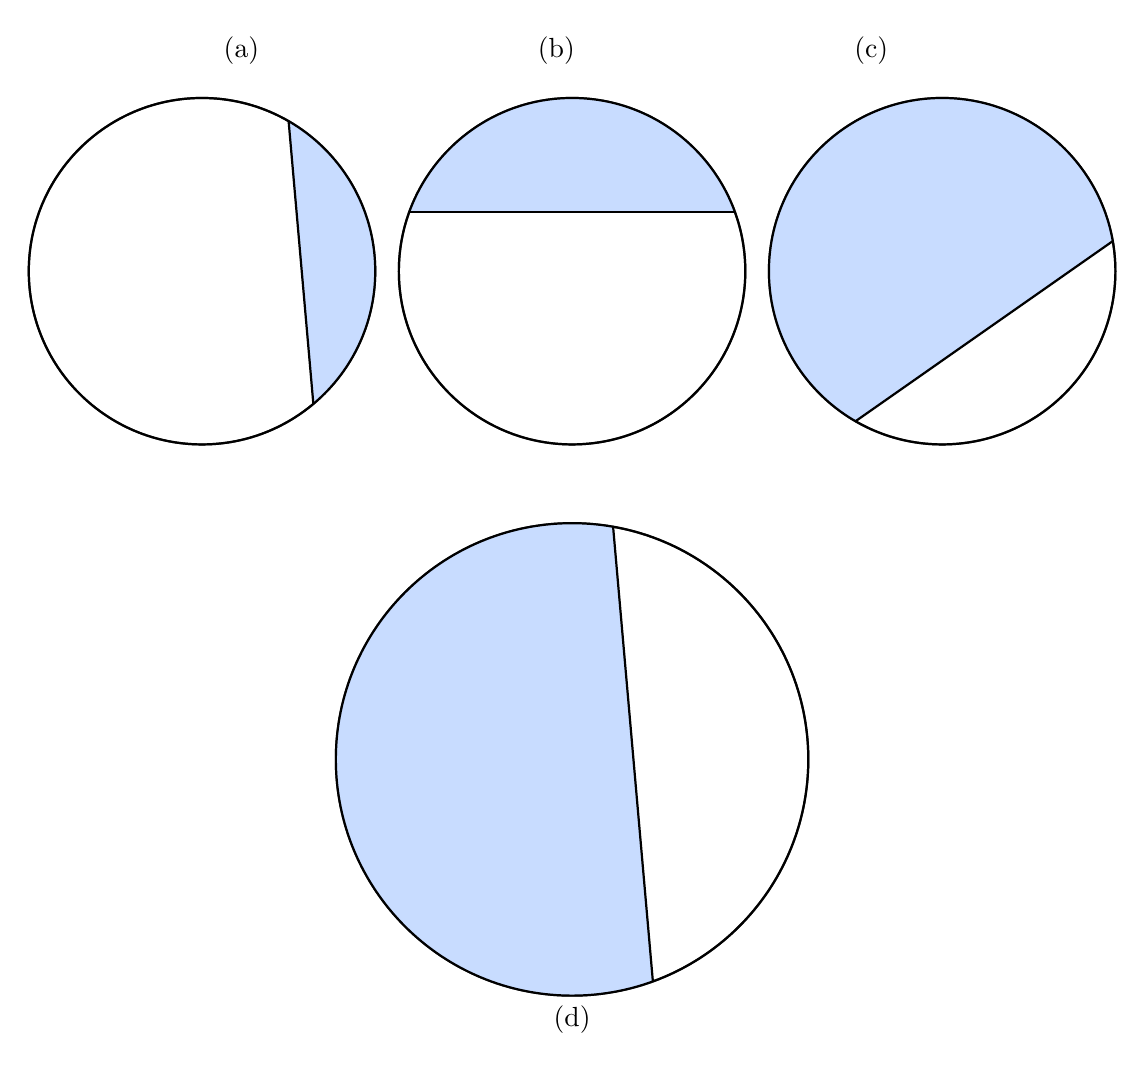
\begin{tikzpicture}[scale=1]
  % a) 1 angle
  \SegmentShaded{-6.5}{0.0}{\Rwork}{-50}{60}{1}{1}{0}{segmentblue}
  \node at (-6.0, -\Rwork+5.0) {(a)};

  % b) 2 angles
  \SegmentShaded{-1.8}{0}{\Rwork}{20}{160}{1}{1}{0}{segmentblue}
  \node at (-2.0, -\Rwork+5.0) {(b)};

  % c) 3 angles
  \SegmentShaded{2.9}{0}{\Rwork}{10}{240}{1}{1}{0}{segmentblue}
  \node at (2.0, -\Rwork+5.0) {(c)};

  % d) 10 angles (larger)
  \SegmentShaded{-1.8}{-6.2}{\Rlarge}{80}{290}{1}{1}{0}{segmentblue}
  \node at (-1.8, -\Rlarge-6.5) {(d)};
\end{tikzpicture}
\end{center}

\textit{Reminder:} Each angle’s vertex must lie on the circumference in the shaded segment

\newpage{}
\vspace{0.5em}

\textbf{3) Interpreting the theorem.}  
For each pair, the \textbf{left} diagram shows two equal angles subtended by the same chord  (\emph{angles in the same segment are equal}). On the \textbf{right}, shade the \textbf{segment and arc} that the theorem refers to.

\begin{center}
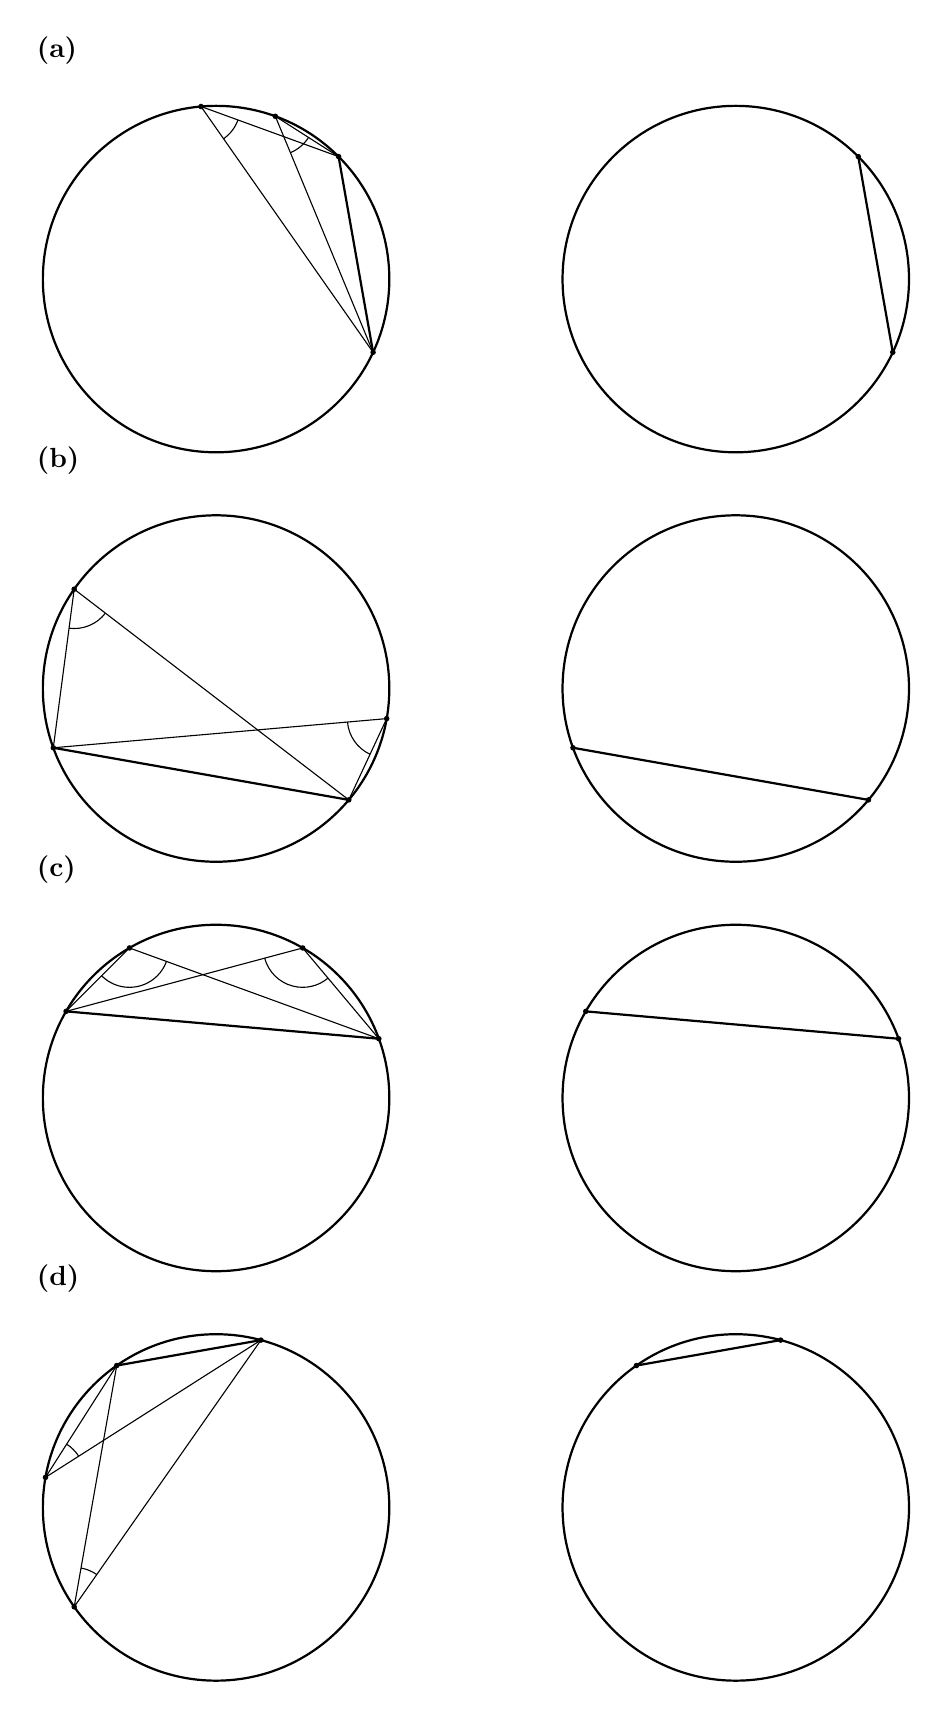
\begin{tikzpicture}[scale=1]
  % (a)
  \TheoremPair{-6.8}{0}{\Rwork}{-25}{45}{70}{95}{6.6}{(a)}
  % (b)
  \TheoremPair{-6.8}{-5.2}{\Rwork}{200}{320}{145}{350}{6.6}{(b)}
  % (c)
  \TheoremPair{-6.8}{-10.4}{\Rwork}{150}{20}{120}{60}{6.6}{(c)}
  % (d)
  \TheoremPair{-6.8}{-15.6}{\Rwork}{75}{125}{170}{215}{6.6}{(d)}
\end{tikzpicture}
\end{center}


\end{document}